%% Wz�ra sprawozdania w LateXu

\documentclass[polish,polish,a4paper]{article}
\usepackage[T1]{fontenc}
\usepackage[cp1250]{inputenc}
\usepackage{babel}
\usepackage{pslatex}
\usepackage{pgfplots}
\usepackage{circuitikz} 
\usepackage{setspace}
\usepackage{caption}
\usepackage{graphicx}
%\usetikzlibrary{circuits.ee.IEC}
\usepackage{anysize}
\marginsize{2.5cm}{2.5cm}{2cm}{2cm}

\newcommand{\PRzFieldDsc}[1]{\sffamily\bfseries\scriptsize #1}
\newcommand{\PRzFieldCnt}[1]{\textit{#1}}
\newcommand{\PRzHeading}[8]{
%% #1 - nazwa laboratorium
%% #2 - kierunek 
%% #3 - specjalno�� 
%% #4 - rok studi�w 
%% #5 - symbol grupy lab.
%% #6 - temat 
%% #7 - numer lab.
%% #8 - sk�ad grupy �wiczeniowej

\begin{center}
\begin{tabular}{ p{0.32\textwidth} p{0.15\textwidth} p{0.15\textwidth} p{0.12\textwidth} p{0.12\textwidth} }

  &   &   &   &   \\
\hline
\multicolumn{5}{|c|}{}\\[-1ex]
\multicolumn{5}{|c|}{{\LARGE #1}}\\
\multicolumn{5}{|c|}{}\\[-1ex]

\hline
\multicolumn{2}{|l|}{\PRzFieldDsc{Kierunek}}	& \multicolumn{2}{|l|}{\PRzFieldDsc{Specjalno��}}	& \multicolumn{1}{|l|}{\PRzFieldDsc{Rok studi�w}}\\
\multicolumn{2}{|c|}{\PRzFieldCnt{#2}}		& \multicolumn{2}{|c|}{\PRzFieldCnt{#3}}		& \multicolumn{1}{|c|}{\PRzFieldCnt{#4}} \\

\hline
\multicolumn{4}{|l|}{\PRzFieldDsc{Temat Laboratorium}}		& \multicolumn{1}{|l|}{\PRzFieldDsc{Numer lab.}} \\
\multicolumn{4}{|c|}{\PRzFieldCnt{#6}}				& \multicolumn{1}{|c|}{\PRzFieldCnt{#7}} \\

\hline
\multicolumn{5}{|l|}{\PRzFieldDsc{Sk�ad grupy �wiczeniowej oraz numery indeks�w}}\\
\multicolumn{5}{|c|}{\PRzFieldCnt{#8}}\\

\hline
\multicolumn{3}{|l|}{\PRzFieldDsc{Uwagi}}	& \multicolumn{2}{|l|}{\PRzFieldDsc{Ocena}} \\
\multicolumn{3}{|c|}{\PRzFieldCnt{\ }}		& \multicolumn{2}{|c|}{\PRzFieldCnt{\ }} \\

\hline
\end{tabular}
\end{center}
}

\begin{document}

\begin{spacing}{1,5}
	
	\begin{figure}[h]
		\centering
		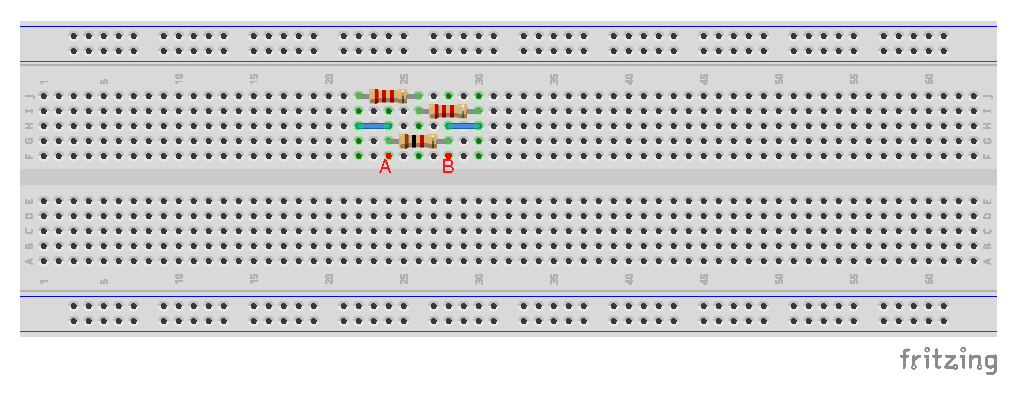
\includegraphics[scale=0.9]{a_bbc.pdf}
		\caption{obw�d (a)}
	\end{figure}

	\begin{figure}[h]
	\centering
	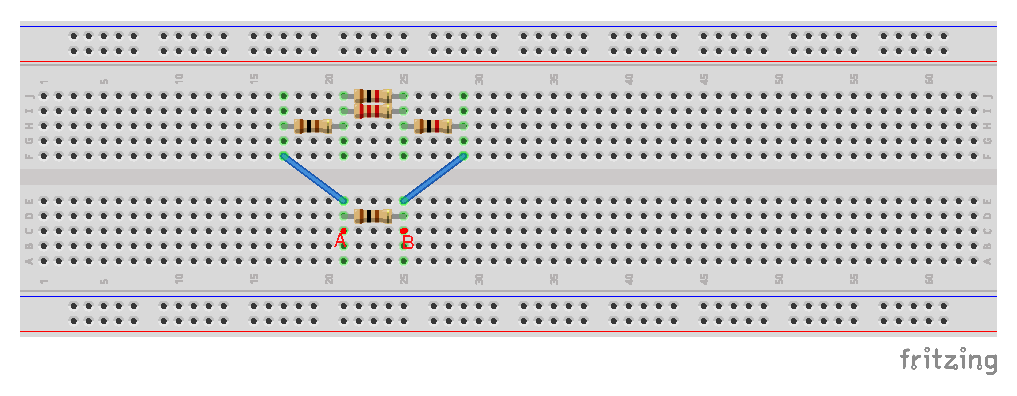
\includegraphics[scale=0.9]{b_bbc.pdf}
	\caption{obw�d (b)}
\end{figure}

	\begin{figure}[h]
	\centering
	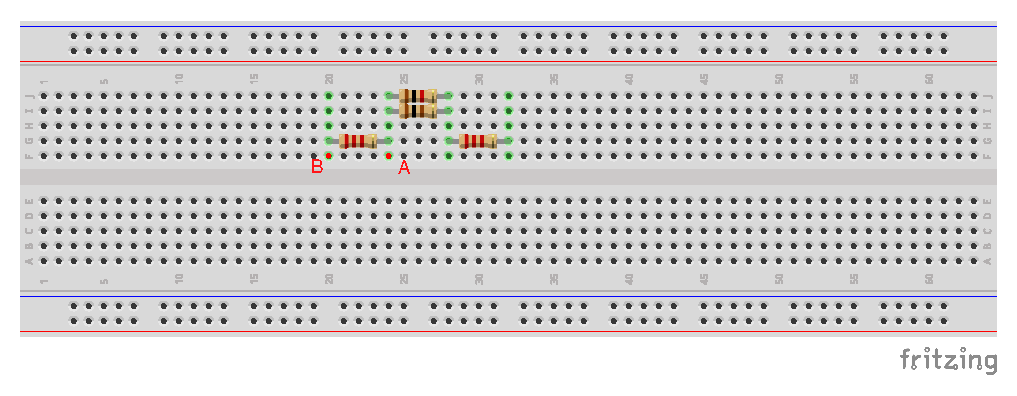
\includegraphics[scale=0.9]{c_bbc.pdf}
	\caption{obw�d (c)}
\end{figure}

	\begin{figure}[h]
	\centering
	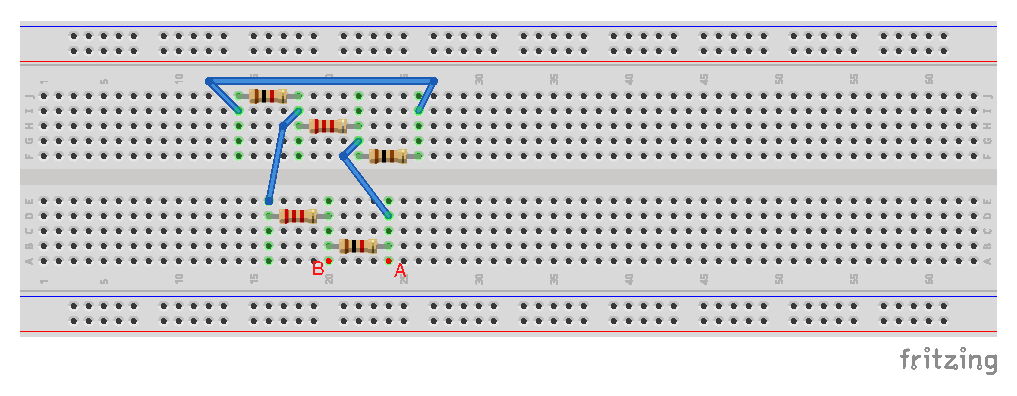
\includegraphics[scale=0.9]{d_bbc.pdf}
	\caption{obw�d (d)}
\end{figure}

	\begin{figure}[h]
	\centering
	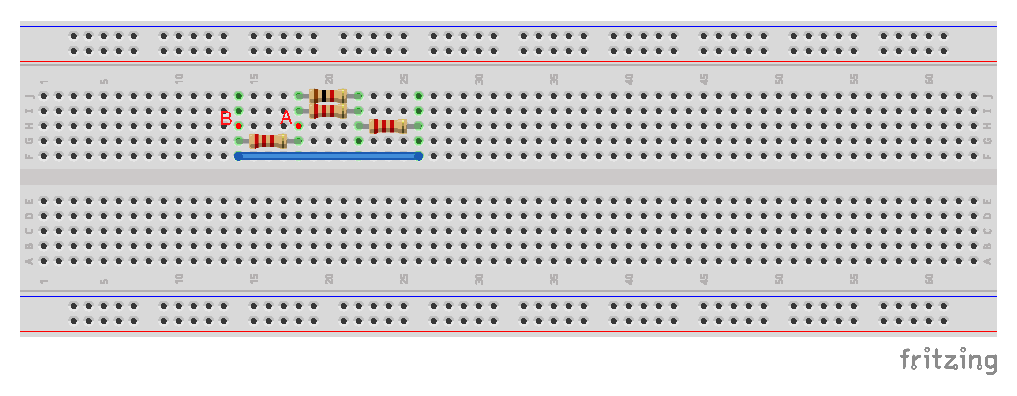
\includegraphics[scale=0.9]{e_bbc.pdf}
	\caption{obw�d (e)}
\end{figure}

	\begin{figure}[h]
	\centering
	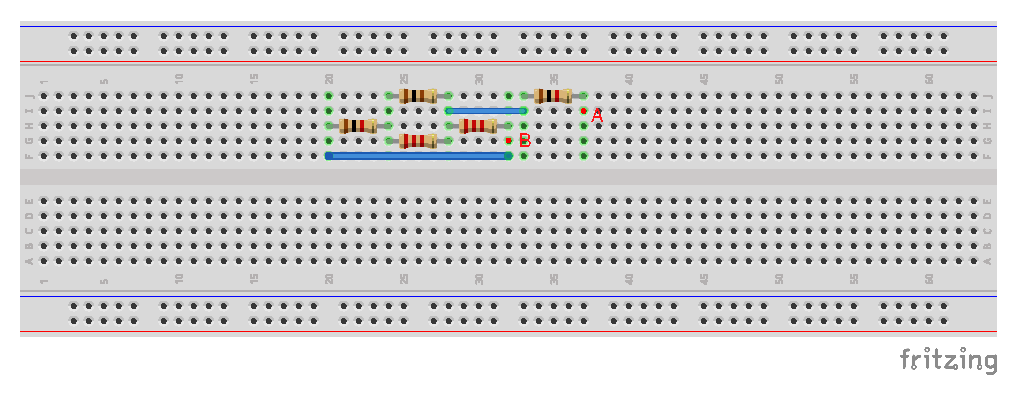
\includegraphics[scale=0.9]{f_bbc.pdf}
	\caption{obw�d (f)}
\end{figure}

\end{spacing}
\end{document}


